\chapter{Introduction} \label{ch1_heading}
% put these two lines after every \chapter{} command

\startarabicpagenumbering % must be just after the first \chapter{} command

%%%%%%%%%%%%%%%%%%%%%%%%%%%%%%%%%%%%%%%%
%%%%% Actual start of Introduction %%%%%
%%%%%%%%%%%%%%%%%%%%%%%%%%%%%%%%%%%%%%%%

With increasingly sophisticated financial industries, so too has the nature of financial crime become more sophisticated. Over the years, financial institutions could construct and combine different processes and technologies that would help combat financial crime. However, by integrating these critical infrastructure elements, financial intuitions are still incapable of entirely grasping the complexity of financial crime. Therefore, financial crime remains a serious complication. A survey conducted in 2018 estimated that the total turnover losses due to financial crime (from the 2373 counties surveyed worldwide) are USD\ 1.45 trillion. More specifically, it is estimated that the total turnover losses due to money laundering are USD\ 267 billion \citep*{begolli2019revealing}. These statistics are astounding, however, financial losses are only one of the consequences of financial crime. Money laundering has several other economic consequences, such as undermining the legitimate private sector and the integrity of financial markets, loss of economic policy, economic distortion and instability, etc. In addition, the social consequences of money laundering are that they financially support crimes such as drug and human trafficking. Therefore, criminals gain the opportunity to expand their operations and adversely impact society \citep*{mcdowell2001consequences}. 

Much has already been done to try and combat the issue of money laundering. \textit{Anti-money laundering} refers to the procedures, laws, and regulations intended to prevent criminals from secretly obtaining illegal funds as a source of legitimate income \citep*{kenton_2021}. Banks are obligated to comply with anti-money laundering regulations. These anti-money laundering compliance programs are enforced due to banks being at high risk to money laundering and other financial crimes \citep*{sanctionscanner}. Therefore, banks specifically design anti-money laundering processes to detect and prevent money laundering. 

In the past few decades, rule-based approaches have been prevalent among banks in dealing with money laundering \citep*{chen2018machine}. These rule-based approaches can either be human-driven or machine-driven. The human or machine-driven mechanisms strive toward one common goal - using client data (historical, transactional, personal, etc.) to develop rules that govern criminals' behaviour. The idea behind a rule-based model is that based on certain transaction scenarios, rules are developed. For the human-driven rule-based approach, domain experts or consultants develop these rules. As the name implies, the machine-driven rule-based approach is when some algorithm does the rule extraction. The rules developed are applied to daily transactions and notify the bank when certain transactions are suspicious. The set of rules is updated if any nuances are identified. Generally, human-driven rule-based approaches are not sufficient to detect financial crimes due to the dynamic nature of criminals, the high volume of data,  and the variety of data that needs to be processed \citep{chen2018machine}. Machine driven rule-based approaches are much more effective in processing huge amounts of financial data. However, the majority of the vanilla rule-based algorithms do not deliver good predictive performance when the rules are applied to new instances. More recently, financial institutions adopted \textit{machine learning} approaches to aid this shortcoming of rule-based approaches. Machine learning is very powerful since it exploits the possibilities of finding an empirical solution to a problem that does not have an analytical solution by using the available data. Therefore, machine learning approaches have the ability to detect complex non-linear patterns in data. Although banks heavily rely on rule-based systems (human and machine-driven) to filter out suspicious transactions, they are partnering with researchers to venture into the feasibility and practicality of implementing machine learning techniques to aid their anti-money laundering processes \citep{chen2018machine}. Examples of machine learning and data mining techniques that have already been applied in a banking context to detect suspicious transactions are outlier detection, support vector machines (SVM), fuzzy logic, clustering, neural networks, genetic algorithms, Bayesian networks, and sequence matching \citep*{al2021financial,abdallah2016fraud, ngai2011application, gao2007framework}. The predominant approach to implementing these techniques consists of using historical transactional data and client-related data to build statistical models that provide a degree of risk of criminal activity. 

\citet*{baesens2015fraud} mentions that networks or graphs give us the ability to map relationships that exists in the real world. For example, if a client makes occasional payments of high amounts to another banking client in a banking context, one might infer some relationship between the two clients. This project will investigate an unconventional approach to help classify the risk of a banking client being involved in any money laundering activity. The project will use complex network analysis and graph theory concepts to extract \textit{network features} or \textit{metric}s from financial data to serve as input to a statistical model. In short, network features describe characteristics of a network or graph's elements (vertices and edges). Also, they  can be the features describing the characteristics of a network as a whole.  Standard machine learning approaches deployed in most anti-money laundering processes do not include network metrics as part of machine learning models inputs. The project aims to establish evidence suggesting that incorporating network metrics in the learning process can be advantageous for conventional anti-money laundering approaches. 

The project will incorporate network metrics to try and capture the relational aspects between banking clients. This relational and other relevant information is provided to a machine learning model as input. Therefore, the network analytic's will function as a feature engineering step.  Emphasis is placed on feature engineering and not data pre-processing.  Although the paper will implement feature engineering and data pre-processing, they represent two different steps. \textit{Feature engineering} is the process of creating features from the data, and \textit{data pre-processing} is the process of altering the data such that it is in a more suitable form for downstream modelling applications \citep*{brownlee_2021, patidar_2021}. Organised crime is a social phenomenon and has a strong relational component attached to it \citep{baesens2015fraud}. Therefore, the project's hypothesis, or premise, is that incorporating these relational components as additional features could improve prediction accuracy, robustness, or both of the machine learning detection models. Figure \ref{fig:ch1_project_framework} illustrates, on a high level, the implementation process of the project. The project has 4 phases (numbered 1-4). The project's first phase generates the raw data (using the AMLSim simulator). Two data sets are primarily used from the simulator's output - the transactional data set and the accounts data set. A pivotal sub-phase is performed upon transitioning from the first phase to the second phase. This sub-phase is the \textit{feature engineering process}. The feature engineering sub-phase generates three structured data tables - \textit{network feature} data table, \textit{transactional feature} data table, and \textit{combined feature} data table. The third phase of the project is the modelling phase which involves the data pre-processing of the structured data, defining the model's architecture, tuning the model hyper-parameters, training the model, and evaluating the model's performance. The results interpretation is the final phase of the project. This phase is concerned with documenting the findings of the project. A more detailed explanation each phase is provided in Chapter \ref{ch3_heading}.   

Many financial crimes exist within a bank, such as credit card fraud, transactional fraud, online banking fraud, etc. However, the project will specifically focus on \textit{money laundering}. The project aims to provide evidence that network metrics/features can improve the performance of machine learning based anti-money laundering processes and essentially aid in the risk profiling of banking clients. The project will investigate how the performance of various classification models are influenced when the inputs to the models consist of i) network features, ii) transactional features,  and iii) network and transactional (combined) features. In short, transactional features are standard features banks use in their risk profiling processes. Also, the data used in the project is synthetically generated using \textit{AMLSim} - a financial transaction simulator developed for research in improving anti-money laundering processes \citep*{AMLSim} . More of the data and how it is generated is mentioned in section \ref{ch3_sub_heading_data}. 

To adequately execute what the project proposes, the following question needs to be considered: 
\begin{center}
\textit{Using historical client transactional data, how can one obtain sufficient evidence that suggests that including network/graph features as inputs to a classification model can improve the classifier's performance in identifying if a banking client is involved in any money laundering activity?}    
\end{center} 

The methodologies used to answer the above question included complex network theory and machine learning. Complex network analysis was used to construct a client network structure and extract network information that gives insight into a client's position and influence ability. On the other hand, the project used machine learning to identify hidden patterns within the data. The thinking behind incorporating the two methodologies was that the network analytics would act as a feature engineering step, generating valuable features for the machine learning model. According to the project's hypothesis, the feature engineering step would ensure that the machine learning model will produce more accurate predictions.  

An outline of the paper is as follows, Chapter \ref{ch2_heading} provides a comprehensive review on the core elements of the project - money laundering, complex network analysis, and machine learning. Next, chapter \ref{ch3_heading} explains the methodology of the project. This chapter is divided into three subsections, explaining sequentially how the data is generated, transformed, and used as input to different classification models. Chapter \ref{ch3_heading} concludes by illustrating the results of the project. Finally, chapter \ref{ch4_heading} discusses the findings of the project as well as recommendations for future work.         

% FCH1_1 - Project framework
\begin{figure}
	\begin{center}
		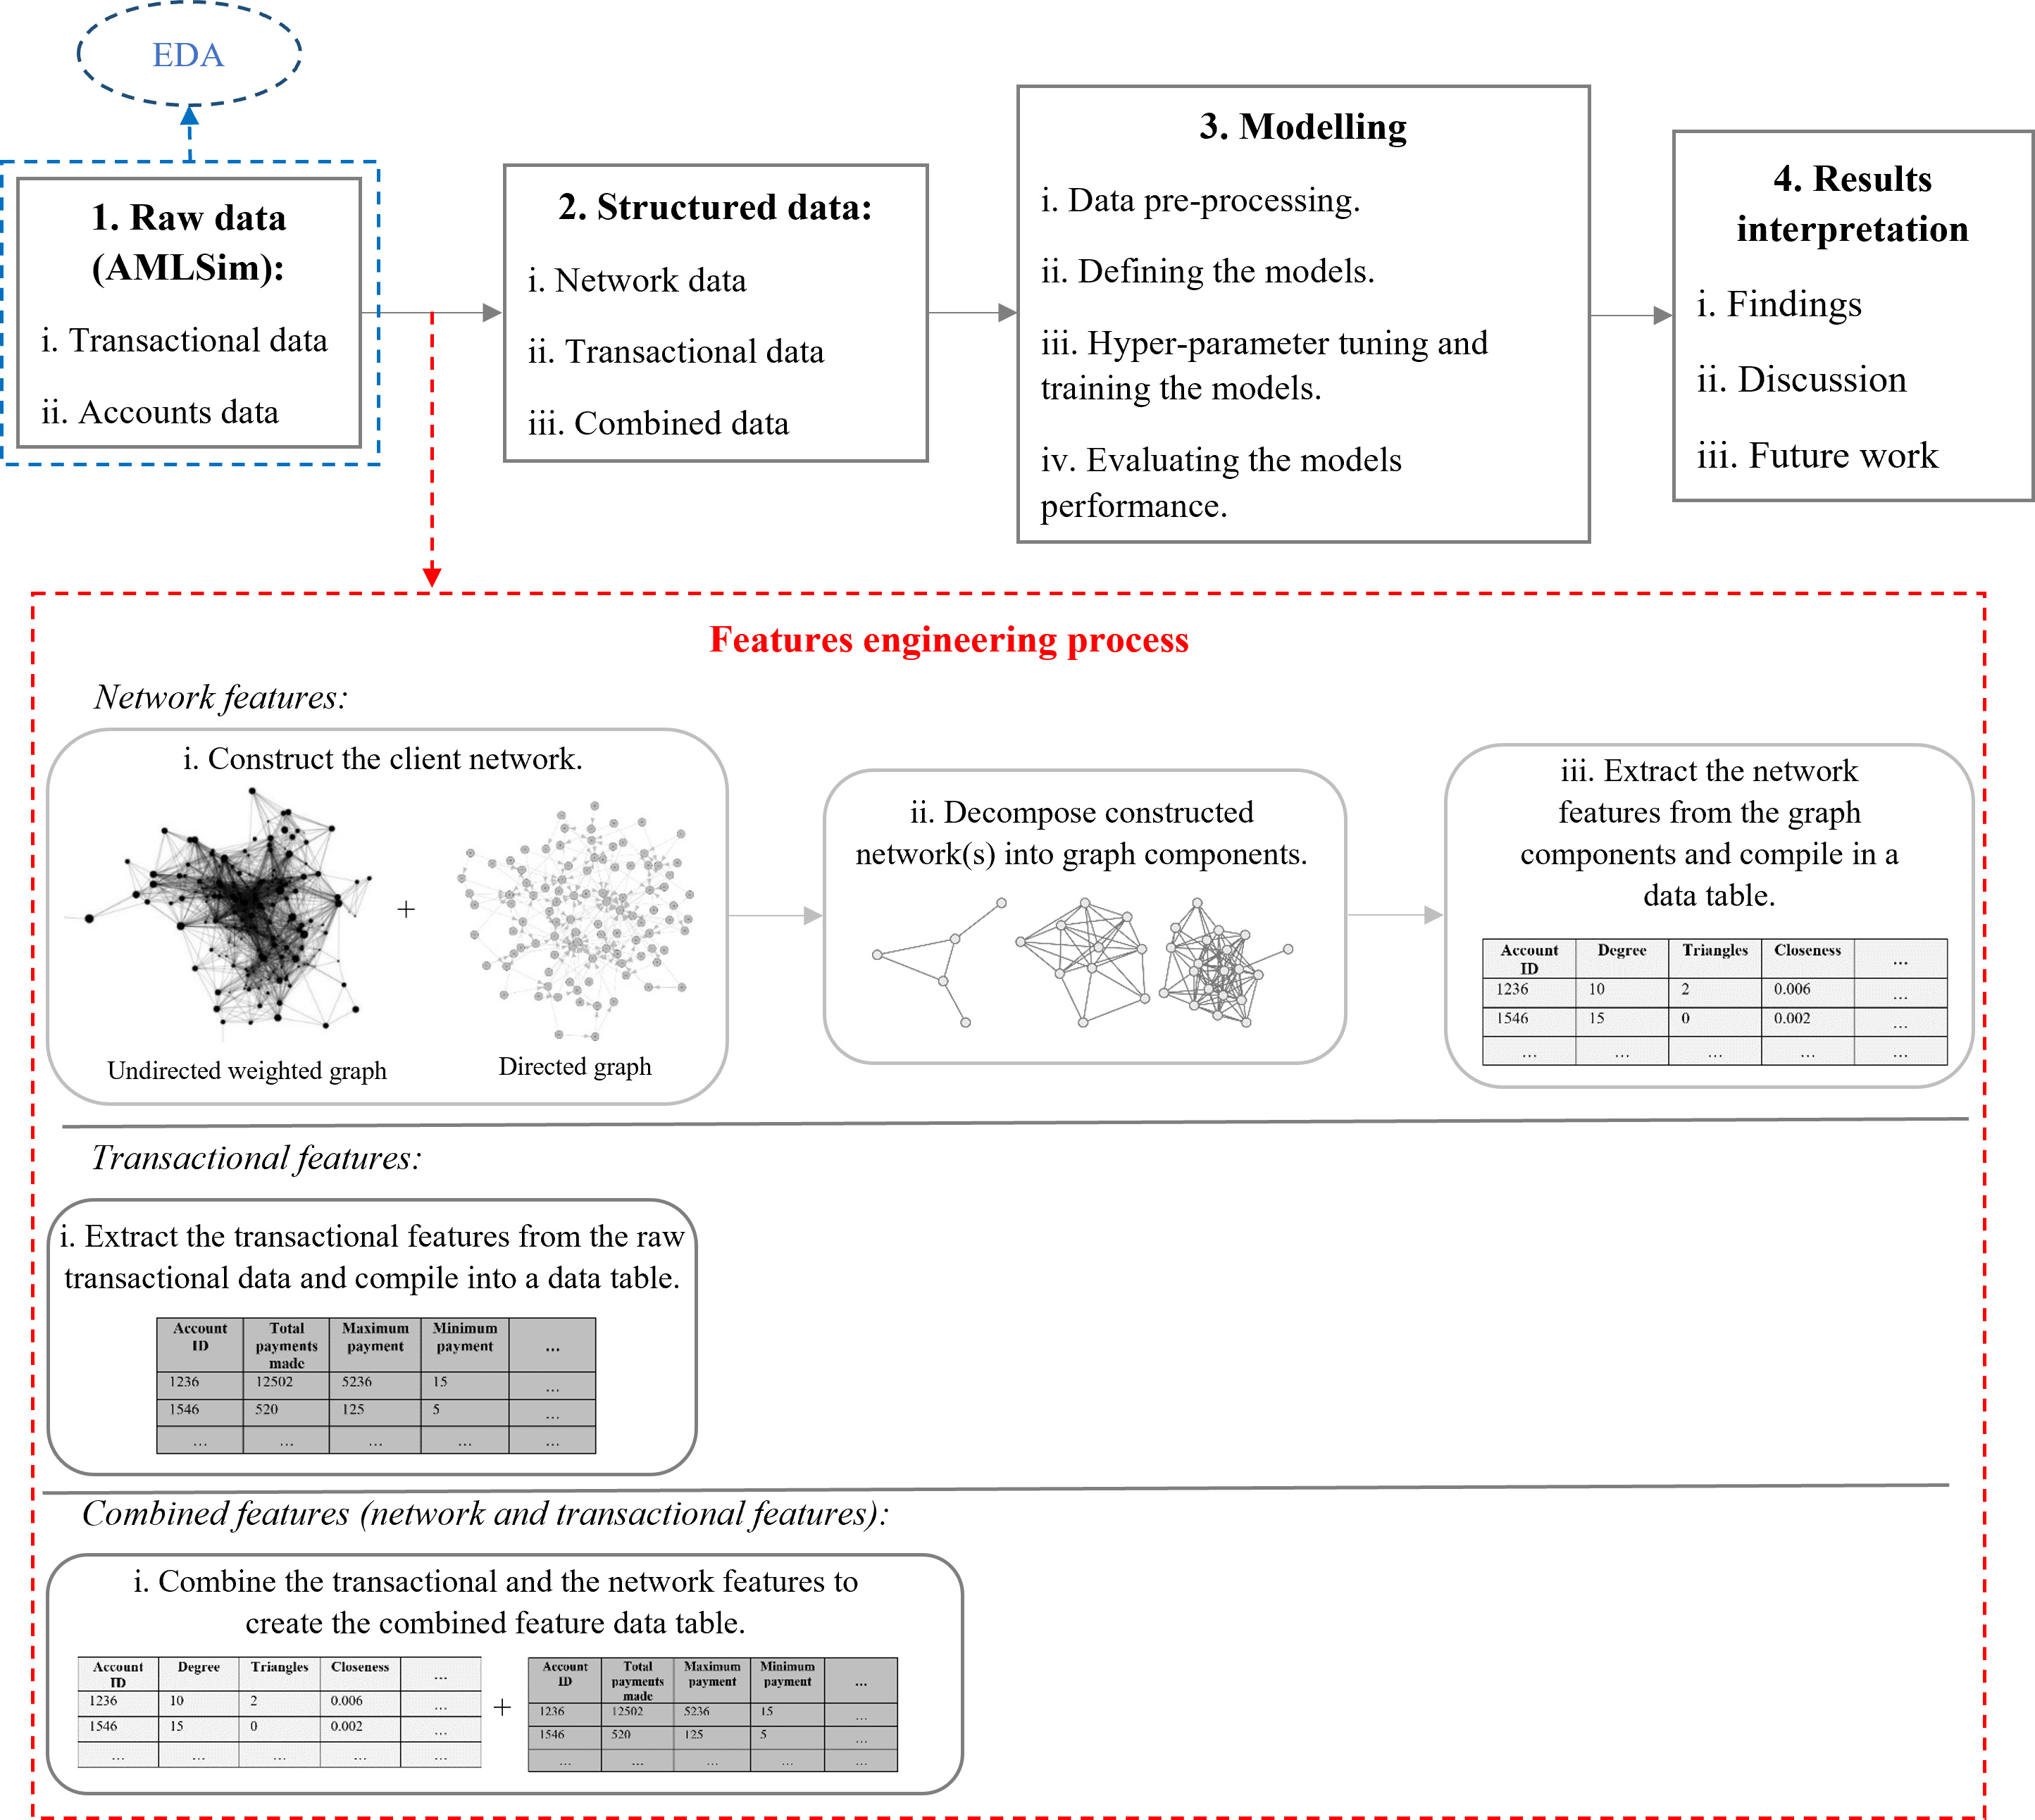
\includegraphics[scale=0.75]{fig/CH1/proposed_project_framework.png}
		\caption{The high-level overview of the implementation of the project. The project has 4 phases (numbered 1-4). The project's first phase generates the raw data (using the AMLSim simulator). The feature engineering process is a sub-phase (between phases one and two) that generates three structured data sets. First, the network feature data table is generated by constructing an undirected weighted network and a directed network. Both networks are constructed from the transactional and accounts raw data (the edges representing the transactions and the vertices the banking accounts). After the networks are constructed, the graph components are extracted. Then, the network features are derived from each component and assigned to each bank account. The second data table is populated by extracting common transactional features for each bank account using the raw transactional information. Lastly, the third data table combines the network feature data table and the transactional feature data table. The third phase of the project is the modelling phase. This phase consists of the modelling procedure implemented in the project. The last phase of the project, the results interpretation phase, is concerned with the project's findings.}
		\label{fig:ch1_project_framework}
	\end{center}	
\end{figure}

